\documentclass[11pt,letterpaper]{article}
\usepackage[lmargin=1in,rmargin=1in,tmargin=1in,bmargin=1in]{geometry}
\usepackage{../style/homework}
\usepackage{../style/commands}
\setbool{quotetype}{true} % True: Side; False: Under
\setbool{hideans}{false} % Student: True; Instructor: False

% -------------------
% Content
% -------------------
\begin{document}

\homework{20: Due 12/15}{The origins of graph theory are humble, even frivolous.}{Norman Biggs}

% Problem 1
\problem{10} Consider the graphs $G$ and $H$ given below. 
	\[
	\begin{tikzpicture}
        \begin{scope}[very thick, decoration= {markings, mark=at position 0.5 with {\arrow{>}}}] 
        
	% Undirected
	\draw[line width=0.05cm, bend left= 30] (-1,1) to (1,1);
	\draw[line width=0.05cm, bend right= 30] (-1,1) to (1,1);
	\draw[line width=0.05cm] (-1,1) to (0,0);
	\draw[line width=0.05cm] (1,1) to (0,0);
	\draw[line width=0.05cm, bend right= 30] (-1,1) to (0,-1);
	\draw[line width=0.05cm, bend left= 30] (1,1) to (0,-1);
	\draw[line width=0.05cm] (0,0) to (0,-1);
	\draw[line width=0.05cm] (0,-1) to (0,-2);
	\draw[line width=0.05cm] (0,-2.3) circle (0.3);
	
	\draw[fill= black] (0,0) circle (0.1);
	\draw[fill= black] (-1,1) circle (0.1);
	\draw[fill= black] (1,1) circle (0.1);
	\draw[fill= black] (0,-1) circle (0.1);
	\draw[fill= black] (0,-2) circle (0.1);
	
	\node at (-1.4,1) {$v_0$};
	\node at (1.4,1) {$v_1$};
	\node at (-0.25,-0.2) {$v_2$};
	\node at (-0.3,-1.1) {$v_3$};
	\node at (-0.25,-1.75) {$v_4$};
	
	\node at (0,1.5) {$e_1$};
	\node at (0,0.9) {$e_2$};
	\node at (-0.9,-0.4) {$e_3$};
	\node at (-0.63,0.35) {$e_4$};
	\node at (0.65,0.35) {$e_5$};
	\node at (0.9,-0.4) {$e_6$};
	\node at (0.25,-1.5) {$e_7$};
	\node at (0.4,-2.7) {$e_8$};
	
	\node at (0,-3.5) {$G$};
	
	% Directed
	\tikzset{shift={(7,-1.2)}}
	\draw[line width= 0.05cm, postaction={decorate}] (-1,1.732) to (1,1.732);
	\draw[line width= 0.05cm, postaction={decorate},bend right= 80] (1,1.732) to (-1,1.732);
	\draw[line width= 0.05cm, postaction={decorate}] (0,0) to (-1,1.732);
	\draw[line width= 0.05cm, postaction={decorate}] (0,0) to (1,1.732);
	\draw[line width=0.05cm, postaction={decorate}] (-1,1.732) arc (0:-360:0.5);
	\draw[line width=0.05cm, postaction={decorate}] (1,1.732) arc (180:540:0.5);
	\draw[line width=0.05cm, postaction={decorate}] (0,0) arc (90:-270:0.5);
	
	
	\draw[fill= black] (-1,1.732) circle (0.1);	
	\draw[fill= black] (0,0) circle (0.1);
	\draw[fill= black] (1,1.732) circle (0.1);
	
	\node at (-0.95,2.3) {$w_1$};
	\node at (0.95,2.3) {$w_2$};
	\node at (0.4,0.1) {$w_3$};
	
	
	\node at (-2.3,1.732) {$f_1$};
	\node at (0,2.65) {$f_2$};
	\node at (0,1.40) {$f_3$};
	\node at (-0.75,0.7) {$f_4$};
	\node at (0.75,0.7) {$f_5$};
	\node at (0,-1.3) {$f_6$};
	\node at (2.4,1.732) {$f_7$};
	
	\node at (0,-2.3) {$H$};
	\end{scope}
	\end{tikzpicture}
	\]

\begin{enumerate}[(a)]
\item Find $\deg v_2$, $\deg v_4$, and $\deg G$.
\item Is $G$ connected? Explain. Is $G$ simple? Explain.
\item Find $\deg^+ \!w_1$ and $\deg^- \!w_1$ as well as $\deg^+ \!w_3$ and $\deg^- \!w_3$. 
\item Find a trail in $H$ that is not a path. 
\item Does $H$ have any sources or sinks? Explain. 
\end{enumerate} \pspace

\sol 
\begin{enumerate}[(a)]
\item The degree of a vertex in an indirected graph is the number of edges incident to the vertex with loops counted twice. Therefore, $\deg v_2= 3$ and $\deg v_4= 3$. The degree of an undirected graph is the sum of the degrees of its vertices. Therefore, we have\dots
	\[
	\deg G= \sum_{v_i} \deg v_i= \deg v_0 + \deg v_1 + \deg v_2 + \deg v_3 + \deg v_4= 4 + 4 + 3 + 4 + 3= 18
	\]
Alternatively, by the Handshake Theorem, the degree of an undirected graph $G$ is twice the number of edges. Therefore, $\deg G= 2 |E(G)|= 2 \cdot 9= 18$. \pspace

\item The graph $G$ is connected because given any two vertices, there is a walk from one vertex to the other. However, the graph $G$ is not simple because there is a loop. Alternatively, the graph $G$ is not simple because there are multiple edges, e.g. there are distinct vertices with more than one edge between them (for instance, there are two edges between $v_0$ and $v_1$). \pspace

\item In a directed graph, the in-degree of a vertex $v$, $\deg^- v$, is the number of edges `coming in' to the vertex. The out-degree of a vertex $v$, $\deg^+ v$, is the number of edges `going out' of the vertex. A loop is counted once in the in and out degree of a vertex. Therefore, $\deg^+ w_1= 2$, $\deg^- w_1= 2$ and $\deg^+ \!w_3= 3$, $\deg^- \!w_3= 1$. \pspace

\item A trail is a walk with no repeated edges whereas a path is a walk where no vertex (and hence no edges) is repeated. Therefore, a trail which is not a path is a walk which does not repeat an edge but does repeat a vertex. For example, $w_1f_3w_2f_2$ is a walk that is a trail but not a path. \pspace

\item In a directed graph, a source is a vertex $v$ with $\deg^- \!v= 0$ while a sink is a vertex $v$ with $\deg^+ \!v= 0$. A vertex with neither of these properties is called interval. Because $\deg^+ \!v \neq 0$ and $\deg^- \!v \neq 0$ for all $v \in V(H)$, there are no sources or sinks in $H$; that is, every vertex in $H$ is internal. 
\end{enumerate}



\newpage



% Problem 2
\problem{10} Suppose you have two graphs, $G$ and $H$, where $G$ is undirected and $H$ may be undirected or directed. The adjacency matrices of $G$ and $H$ are given below. \par
	\def\matrixG{%
	\begin{matrix}
	0 & 1 & 1 & 0 \\
	1 & 1 & 0 & 1 \\
	1 & 0 & 0 & 2 \\
	0 & 1 & 2 & 0 
	\end{matrix}
	}%
	\def\matrixH{%
	\begin{matrix}
	0 & 0 & 1 & 0 & 0 \\
	1 & 0 & 0 & 0 & 0 \\
	0 & 1 & 0 & 0 & 0 \\
	0 & 0 & 0 & 0 & 1 \\
	0 & 0 & 0 & 2 & 0 
	\end{matrix}
	}%
	\[
	\left(\vphantom{\matrixG} \right.\kern-2\nulldelimiterspace
  \underbrace{\matrixG}_{G} \kern-\nulldelimiterspace\left.\vphantom{\matrixG} \right) \qquad
  	\left(\vphantom{\matrixH} \right.\kern-2\nulldelimiterspace
  \underbrace{\matrixH}_{H} \kern-\nulldelimiterspace\left.\vphantom{\matrixH} \right)
	\]

\begin{enumerate}[(a)]
\item Draw the graph of $G$.
\item Does $G$ have a loop? Justify your answer using \textit{only} the adjacency matrix of $G$.
\item Draw the graph of $H$.
\item Is $H$ undirected or directed? Justify your answer using \textit{only} the adjacency matrix of $H$.
\item Do $G$ or $H$ have multiple edges? Explain your answer using only the adjacency matrix of $G$ and $H$, respectively. 
\end{enumerate} \pspace

\sol 
\begin{enumerate}[(a)]
\item We have\dots
	\[
	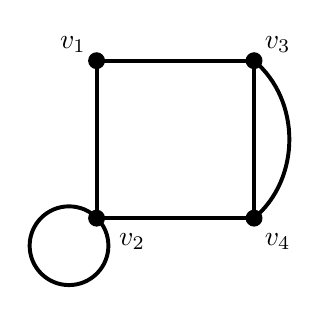
\begin{tikzpicture}
	\draw[line width=0.05cm] (0,0) -- (2,0) -- (2,2) -- (0,2) -- (0,0);
	\draw[line width=0.05cm,bend right= 50] (2,0) to (2,2);
	\draw[line width=0.05cm] (-0.35,-0.35) circle (0.5);
	
	\draw[fill= black] (0,0) circle (0.1);
	\draw[fill= black] (2,0) circle (0.1);
	\draw[fill= black] (2,2) circle (0.1);
	\draw[fill= black] (0,2) circle (0.1);
	
	\node at (0.45,-0.3) {$v_2$};
	\node at (2.3,-0.3) {$v_4$};
	\node at (2.3,2.2) {$v_3$};
	\node at (-0.3,2.2) {$v_1$};
	\end{tikzpicture}
	\] \pspace

\item A loop is an edge from a vertex $v_i$ to itself. But then $G_{i,i} > 0$. Because $G_{2,2} > 0$, there is a loop incident to vertex $v_2$. \pspace

\item We have\dots
	\[
	\begin{tikzpicture}
	\begin{scope}[very thick, decoration= {markings, mark=at position 0.5 with {\arrow{>}}}] 
	\draw[line width= 0.05cm, postaction={decorate}] (0,0) to (1,1.73);
	\draw[line width= 0.05cm, postaction={decorate}] (1,1.73) to (2,0);
	\draw[line width= 0.05cm, postaction={decorate}] (2,0) to (0,0);
	
	\draw[line width= 0.05cm, postaction={decorate}] (3.5,1.73) to (3.5,0);
	\draw[line width= 0.05cm, postaction={decorate}, bend left= 50] (3.5,0) to (3.5,1.73);
	\draw[line width= 0.05cm, postaction={decorate}, bend right= 50] (3.5,0) to (3.5,1.73);
	
	\draw[fill= black] (0,0) circle (0.08);
	\draw[fill= black] (1,1.73) circle (0.08);
	\draw[fill= black] (2,0) circle (0.08);
	\draw[fill= black] (3.5,0) circle (0.08);
	\draw[fill= black] (3.5,1.73) circle (0.08);
	
	\node at (-0.2,-0.3) {$v_2$};
	\node at (1,2.1) {$v_1$};
	\node at (2.2,-0.3) {$v_3$};
	
	\node at (3.5,2.1) {$v_4$};
	\node at (3.5,-0.35) {$v_5$};
	\end{scope}
	\end{tikzpicture}
	\] \pspace

\item If a graph is undirected, then its adjacency matrix is symmetric, i.e. $A^T= A$. But then $a_{ij}= a_{ji}$ for all $i, j$. By contrapositive, if the adjacency matrix for a graph is not symmetric, then the graph cannot eb directed. Observe that the adjacency matrix for $H$ is not symmetric. For instance, $H_{2,1}= 1 \neq 0= H_{1,2}$. Therefore, $H$ is a directed graph. 

\item A graph has multiple edges if there exist two distinct vertices with more than one edge between them. But then if $A$ is the adjacency matrix for the graph, then $a_{ij} > 1$ for some $i, j$. Because $G_{3,4}= 2 > 1$ and $H_{5,4}= 2 > 1$, both $G$ and $H$ have multiple edges. 
\end{enumerate}



\newpage



% Problem 3
\problem{10} Showing all your work and fully justifying your responses, complete the following:
	\begin{enumerate}[(a)]
	\item Draw the graph of $K_5$. How many vertices and edges does $K_5$ have? For $n \geq 1$, what are $|V(K_n)|$ and $|E(K_n)|$?
	\item Draw the graph of $K_{3, 5}$. How many vertices and edges does $K_{3, 5}$ have? For $m, n \geq 1$, what are $|V(K_{m, n})|$ and $|E(K_{m, n})|$?
	\item If $G$ is a simple graph, the complement of $G$, denoted $\widetilde{G}$, is a graph with $V(G)= V(\widetilde{G})$ and two vertices are adjacent in $\widetilde{G}$ if and only if they are not adjacent in $G$. Find the complement of the graph given below. Is $G$ connected? Is $\widetilde{G}$ connected? 
		\[
		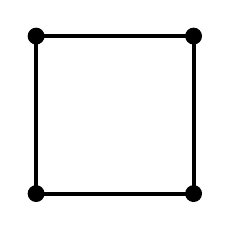
\begin{tikzpicture}[scale=2]
		\draw[line width= 0.05cm] (0,0) -- (1,0) -- (1,1) -- (0,1) -- (0,0);
		
		\draw[fill=black] (0,0) circle (0.05); 
		\draw[fill=black] (1,0) circle (0.05); 
		\draw[fill=black] (1,1) circle (0.05); 
		\draw[fill=black] (0,1) circle (0.05); 
		\end{tikzpicture}
		\]
	\end{enumerate} \pspace

\sol 
\begin{enumerate}[(a)]
\item We have\dots
	\[
	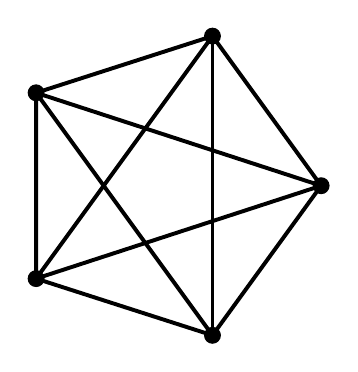
\begin{tikzpicture}[scale=1]
	\draw[line width= 0.05cm] (2,0) -- (0.62,1.9) -- (-1.62,1.18) -- (-1.62,-1.18) -- (0.62,-1.9) -- (2,0);
	\draw[line width= 0.05cm] (2,0) -- (-1.62,1.18);
	\draw[line width= 0.05cm] (2,0) -- (-1.62,-1.18);
	\draw[line width= 0.05cm] (0.62,1.9) -- (-1.62,-1.18);
	\draw[line width= 0.05cm] (0.62,1.9) -- (0.62,-1.9);
	\draw[line width= 0.05cm] (-1.62,1.18) -- (0.62,-1.9);
	
	\draw[fill=black] (2,0) circle (0.1); 
	\draw[fill=black] (0.62,1.9) circle (0.1); 
	\draw[fill=black] (-1.62,1.18) circle (0.1); 
	\draw[fill=black] (-1.62,-1.18) circle (0.1); 
	\draw[fill=black] (0.62,-1.9) circle (0.1); 
	\end{tikzpicture}
	\]
This graph has 5 vertices and 10 edges. In general, to draw $K_n$, we first place $n$ vertices. Therefore, $|V(K_n)|= n$. We then have an edge between every distinct pair of vertices. But then the number of edges is the number of ways of selecting any two distinct pair of vertices. There are $\binom{n}{2}= \dfrac{n(n - 1)}{2}$ ways of choosing any distinct pair of vertices. Therefore, we have $|E(K_n)|= \binom{n}{2}= \dfrac{n(n - 1)}{2}$. Alternatively, we can draw an edge between every (not necessarily distinct) vertex. There are $n \cdot n= n^2$ such edges. But then we have also drawn $n$ loops (one at each vertex)---which are not in $K_n$. Removing these loops, we then have $n^2 - n$ edges. However, once one has drawn a edge from one vertex to another, one need not draw it `the other way.' We have then doubles the amount of edges in $K_n$. Therefore, the number of edges is $\frac{1}{2} \cdot (n^2- n)= \dfrac{n^2 - n}{2}= \dfrac{n(n - 1)}{2}$. 

\item We have\dots
	\[
	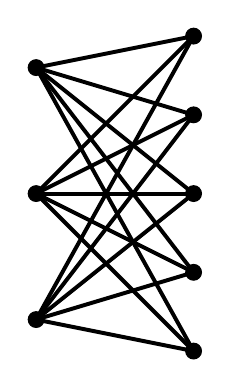
\begin{tikzpicture}[scale=1]
	\draw[line width= 0.05cm] (0,0.4) -- (2,0);
	\draw[line width= 0.05cm] (0,0.4) -- (2,1);
	\draw[line width= 0.05cm] (0,0.4) -- (2,2);
	\draw[line width= 0.05cm] (0,0.4) -- (2,3);
	\draw[line width= 0.05cm] (0,0.4) -- (2,4);
	\draw[line width= 0.05cm] (0,2.0) -- (2,0);
	\draw[line width= 0.05cm] (0,2.0) -- (2,1);
	\draw[line width= 0.05cm] (0,2.0) -- (2,2);
	\draw[line width= 0.05cm] (0,2.0) -- (2,3);
	\draw[line width= 0.05cm] (0,2.0) -- (2,4);
	\draw[line width= 0.05cm] (0,3.6) -- (2,0);
	\draw[line width= 0.05cm] (0,3.6) -- (2,1);
	\draw[line width= 0.05cm] (0,3.6) -- (2,2);
	\draw[line width= 0.05cm] (0,3.6) -- (2,3);
	\draw[line width= 0.05cm] (0,3.6) -- (2,4);
	
	\draw[fill=black] (0,0.4) circle (0.1); 
	\draw[fill=black] (0,2.0) circle (0.1); 
	\draw[fill=black] (0,3.6) circle (0.1); 
	
	\draw[fill=black] (2,0) circle (0.1); 
	\draw[fill=black] (2,1) circle (0.1); 	
	\draw[fill=black] (2,2) circle (0.1); 
	\draw[fill=black] (2,3) circle (0.1); 
	\draw[fill=black] (2,4) circle (0.1); 
	\end{tikzpicture}
	\]
This graph has 8 vertices and 15 edges. In general, to draw $K_{m,n}$, we must first draw a collection of $m$ vertices and a collection of $n$ vertices. But then there are $m + n$ vertices, i.e. $|V(K_{m,n})|= m + n$. For each of the $m$ vertices in the `first' collection, we need to draw an edge to each of the $n$ vertices in the `other' collection of vertices. But then there are $m \cdot n$ total edges, i.e. $|E(K_{m,n})|= mn$. \pspace

\item The complement of the graph is\dots
	\[
	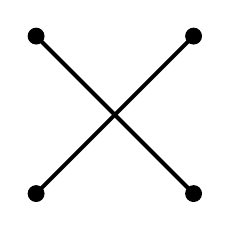
\begin{tikzpicture}[scale=2]
	\draw[line width= 0.05cm] (0,0) -- (1,1);
	\draw[line width= 0.05cm] (0,1) -- (1,0);
	
	\draw[fill=black] (0,0) circle (0.05); 
	\draw[fill=black] (1,0) circle (0.05); 
	\draw[fill=black] (1,1) circle (0.05); 
	\draw[fill=black] (0,1) circle (0.05); 
	\end{tikzpicture}
	\]
Observe that original graph $G$ is connected because there is a walk between every pair of vertices. However, $\widetilde{G}$ is not connected because there is not a walk between each pair of vertices. Although, it may look like this is the case with how the graph is drawn above. There is no vertex at the intersection of edges above. We could have drawn the complement as below to emphasize that the graph is disconnected:
	\[
	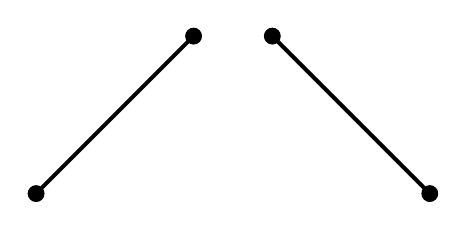
\begin{tikzpicture}[scale=2]
	\draw[line width= 0.05cm] (0,0) -- (1,1);
	\draw[line width= 0.05cm] (1.5,1) -- (2.5,0);
	
	\draw[fill=black] (0,0) circle (0.05); 
	\draw[fill=black] (1.5,1) circle (0.05); 
	\draw[fill=black] (1,1) circle (0.05); 
	\draw[fill=black] (2.5,0) circle (0.05); 
	\end{tikzpicture}
	\]
\end{enumerate}



\newpage



% Problem 4
\problem{10} Below are three graphs: $G_1$, $G_2$, and $G_3$. Determine which, if any, of the graphs are isomorphic. If two given graphs are isomorphic, show that they are isomorphic. If two graphs are not isomorphic, give at least two reasons why they are not isomorphic. 
	\[
	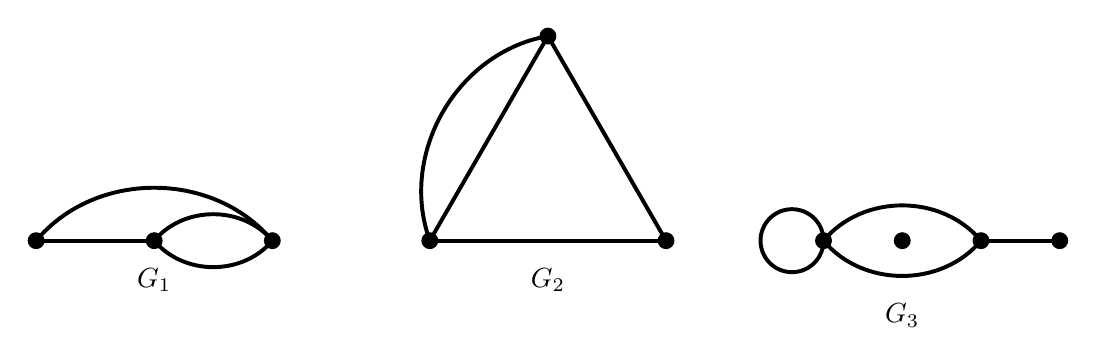
\begin{tikzpicture}
	% Graph 1
	\draw[line width=0.05cm] (0,0) -- (1.5,0);
	\draw[line width=0.05cm, bend left= 50] (1.5,0) to (3,0);
	\draw[line width=0.05cm, bend right= 50] (1.5,0) to (3,0);
	\draw[line width=0.05cm, bend left= 50] (0,0) to (3,0);

	\draw[fill=black] (0,0) circle (0.1); 
	\draw[fill=black] (1.5,0) circle (0.1); 
	\draw[fill=black] (3,0) circle (0.1); 
	
	\node at (1.5, -0.5) {$G_1$}; 
	
	% Graph 2
	\tikzset{shift={(5,0)}}
	
	\draw[line width=0.05cm] (0,0) to (1.5,2.598);
	\draw[line width=0.05cm, bend left= 50] (0,0) to (1.5,2.598);
	\draw[line width=0.05cm] (1.5,2.598) to (3,0);
	\draw[line width=0.05cm] (0,0) to (3,0);

	\draw[fill=black] (0,0) circle (0.1); 
	\draw[fill=black] (1.5,2.598) circle (0.1); 
	\draw[fill=black] (3,0) circle (0.1); 
	
	\node at (1.5,-0.5) {$G_2$};
	
	% Graph 3
	\tikzset{shift={(5,0)}}
	
	\draw[line width=0.05cm] (-0.4,0) circle (0.4);
	\draw[line width=0.05cm, bend left= 50] (0,0) to (2,0);
	\draw[line width=0.05cm, bend right= 50] (0,0) to (2,0);
	\draw[line width=0.05cm] (2,0) to (3,0);
		
	\draw[fill=black] (0,0) circle (0.1);
	\draw[fill=black] (1,0) circle (0.1);
	\draw[fill=black] (2,0) circle (0.1);
	\draw[fill=black] (3,0) circle (0.1);
	
	\node at (1.0,-0.95) {$G_3$};
	\end{tikzpicture}
	\] 

\sol First, observe that $G_1$ is isomorphic to $G_2$ because we can slowly transform one graph into the other:
	\[
	\begin{tikzpicture}[
	>=stealth',
	pos=.8,
	curvy/.style={decorate,decoration={snake,post length=1mm}}
	]
	% Graph 1
	\draw[line width=0.05cm] (0,0) -- (1.5,0);
	\draw[line width=0.05cm, bend left= 50] (1.5,0) to (3,0);
	\draw[line width=0.05cm, bend right= 50] (1.5,0) to (3,0);
	\draw[line width=0.05cm, bend left= 50] (0,0) to (3,0);

	\draw[fill=black] (0,0) circle (0.1); 
	\draw[fill=black] (1.5,0) circle (0.1); 
	\draw[fill=black] (3,0) circle (0.1); 
	
	% Second
	\draw[line width=0.05cm,curvy,->] (4,0) -- (5,0);
	\tikzset{shift={(4.5,0)}}
	
	\draw[line width=0.05cm, bend left= 50] (1.5,0) to (3,0);
	\draw[line width=0.05cm, bend right= 50] (1.5,0) to (3,0);
	\draw[line width=0.05cm] (3,0) to (4.5,0);
	\draw[line width=0.05cm, bend right= 50] (4.5,0) to (1.5,0);
	
	\draw[fill=black] (1.5,0) circle (0.1); 
	\draw[fill=black] (3,0) circle (0.1); 
	\draw[fill=black] (4.5,0) circle (0.1); 
	
	% Third
	\draw[line width=0.05cm,curvy,->] (5.5,0) -- (6.5,0);
	\tikzset{shift={(8,-1)}}

	\draw[line width=0.05cm] (0,0) to (1.5,2.598);
	\draw[line width=0.05cm, bend left= 50] (0,0) to (1.5,2.598);
	\draw[line width=0.05cm] (1.5,2.598) to (3,0);
	\draw[line width=0.05cm] (0,0) to (3,0);

	\draw[fill=black] (0,0) circle (0.1); 
	\draw[fill=black] (1.5,2.598) circle (0.1); 
	\draw[fill=black] (3,0) circle (0.1); 
	\end{tikzpicture}
	\]
Alternatively, label the graphs $G_1$ and $G_2$ as below:
	\[
	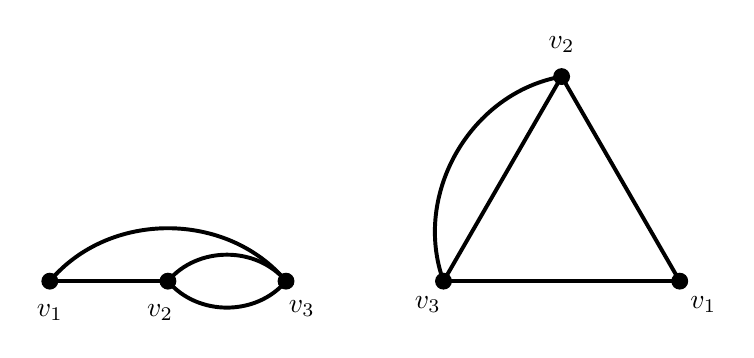
\begin{tikzpicture}
	\draw[line width=0.05cm] (0,0) -- (1.5,0);
	\draw[line width=0.05cm, bend left= 50] (1.5,0) to (3,0);
	\draw[line width=0.05cm, bend right= 50] (1.5,0) to (3,0);
	\draw[line width=0.05cm, bend left= 50] (0,0) to (3,0);

	\draw[fill=black] (0,0) circle (0.1); 
	\draw[fill=black] (1.5,0) circle (0.1); 
	\draw[fill=black] (3,0) circle (0.1); 
	
	\node at (0,-0.4) {$v_1$};
	\node at (1.4,-0.4) {$v_2$};
	\node at (3.2,-0.35) {$v_3$};
	
	\tikzset{shift={(5,0)}}
	
	\draw[line width=0.05cm] (0,0) to (1.5,2.598);
	\draw[line width=0.05cm, bend left= 50] (0,0) to (1.5,2.598);
	\draw[line width=0.05cm] (1.5,2.598) to (3,0);
	\draw[line width=0.05cm] (0,0) to (3,0);

	\draw[fill=black] (0,0) circle (0.1); 
	\draw[fill=black] (1.5,2.598) circle (0.1); 
	\draw[fill=black] (3,0) circle (0.1); 
	
	\node at (-0.2,-0.3) {$v_3$};
	\node at (3.3,-0.3) {$v_1$};
	\node at (1.5,3) {$v_2$};
	\end{tikzpicture}
	\]
Observe that both graphs then have the following adjacency matrix:
	\[
	\begin{pmatrix}
	0 & 1 & 1 \\
	1 & 0 & 2 \\
	1 & 2 & 0 
	\end{pmatrix}
	\]
Two graphs are isomorphic if and only if they have the same adjacency matrix for some labeling of their vertices. But then the work above shows that $G_1$ is isomorphic to $G_2$. \pspace

Now $G_3$ cannot be isomorphic to $G_1$ or $G_2$. The number of vertices a graph has is invariant under isomorphism. Because $G_3$ has four vertices, i.e. $|V(G_3)|= 4$, and $G_1, G_2$ have three vertices, i.e. $|V(G_1)|= |V(G_2)|= 3$, $G_3$ cannot be isomorphic to $G_1$ or $G_2$. Furthermore, the number of loops a graph has is invariant under isomorphism. But because $G_3$ has a loop while $G_1$ and $G_2$ do not, $G_3$ cannot be isomorphic to $G_1$ or $G_2$. Furthermore, the degrees of vertices is invariant under isomorphism. Because $G_3$ has a vertex of degree 4 (the `leftmost' vertex) while $G_1$ and $G_2$ do not have a vertex of degree 4, $G_3$ cannot be isomorphic to $G_1$ or $G_2$. Furthermore, the number of isolated vertices is invariant under isomorphism. Because $G_3$ has one isolated vertex while $G_1$ and $G_3$ have none, $G_3$ cannot be isomorphic to $G_1$ or $G_2$. 


\end{document}